\documentclass{beamer}

% fonts
\usepackage[utf8]{inputenc}
\usepackage[francais]{babel}

% asm
\usepackage{amsmath}
\usepackage{amssymb}
\usepackage{amsthm}

% diagrams
\usepackage{tikz}
\usetikzlibrary{matrix}
\usetikzlibrary{positioning}

% titlepage
\title{Lattice Reduction Techniques\\To Attack RSA}
\author{David Wong}
\institute{University of Bordeaux}
\date{March 2015}
\setbeamercolor*{title}{fg=white}
\setbeamercolor*{author}{fg=white}
\setbeamercolor*{institute}{fg=white}
\setbeamercolor*{date}{fg=white}

%
\begin{document}

% TITLE
\fontsize{16pt}{15.2}\selectfont
\usebackgroundtemplate{
\includegraphics[width=\paperwidth,height=\paperheight]{img/blurry.jpg}} 
\begin{frame}
\titlepage
\end{frame}

% RSA
\fontsize{90pt}{15.2}\selectfont
\usebackgroundtemplate{
\includegraphics[width=\paperwidth,height=\paperheight]{img/blurry2.jpg}}
\begin{frame}
\begin{center}
\textbf{RSA?}
\end{center}
\end{frame}

% ENCRYPT/DECRYPT
\fontsize{14pt}{15.2}\selectfont
\usebackgroundtemplate{}
\begin{frame}
$(e, N)$ is the \textbf{public key}, 
$(d, N)$ is the \textbf{private key}.\\

\pause

\vspace{1cm} To \textbf{encrypt} a message $m$, with $m < N$ we just do:
\[ c = m^e \pmod{N} \]
\pause
And to \textbf{decrypt}:
\[ m = c^d \pmod{N} \]
\end{frame}

\begin{frame}
To generate these keys, we first generate \textbf{two primes} $p$ and $q$ such that:
\[ N = p \times q \]
\pause
Use $p$ and $q$ to generate the pair \textbf{private key/public key} $(d,e)$.
\end{frame}

% ATTACKS?
\fontsize{90pt}{15.2}\selectfont
\usebackgroundtemplate{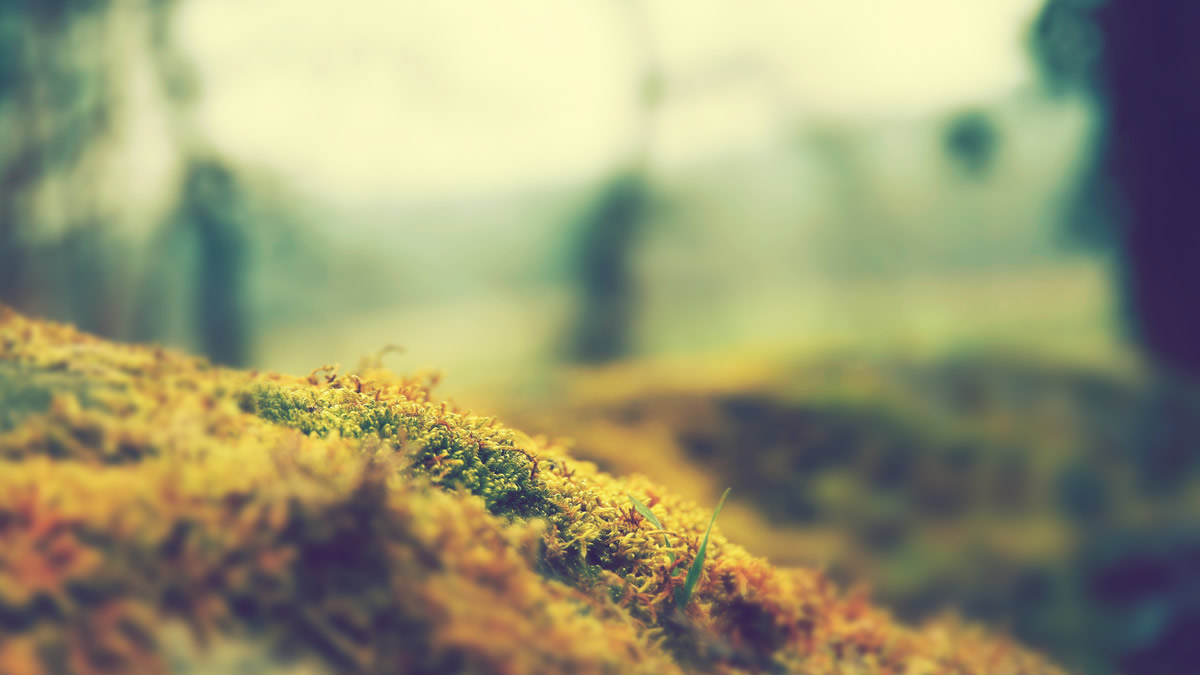
\includegraphics[width=\paperwidth,height=\paperheight]{img/blurry3.jpg}}
\begin{frame}
\begin{center}

\textbf{ATTACKS?}
\end{center}
\end{frame}

%
\fontsize{14pt}{15.2}\selectfont
\usebackgroundtemplate{}
\begin{frame}

On the implementation or on the mathematics.\\\vspace{1cm}
\pause
 \textbf{Model}:

\begin{itemize}
	\item{Recover the plaintext $m^e = c \pmod{N}$}
	\item{Recover the private key $d$}
\end{itemize}
\vspace{1cm}
\pause
\textbf{Relaxed model}:
\pause
\begin{itemize}
	\item{We know a part of the message}
	\item{We know an approximation of one of the prime}
	\item{The private exponent is too small}
\end{itemize}
\end{frame}

% LATTICE
\fontsize{90pt}{15.2}\selectfont
\usebackgroundtemplate{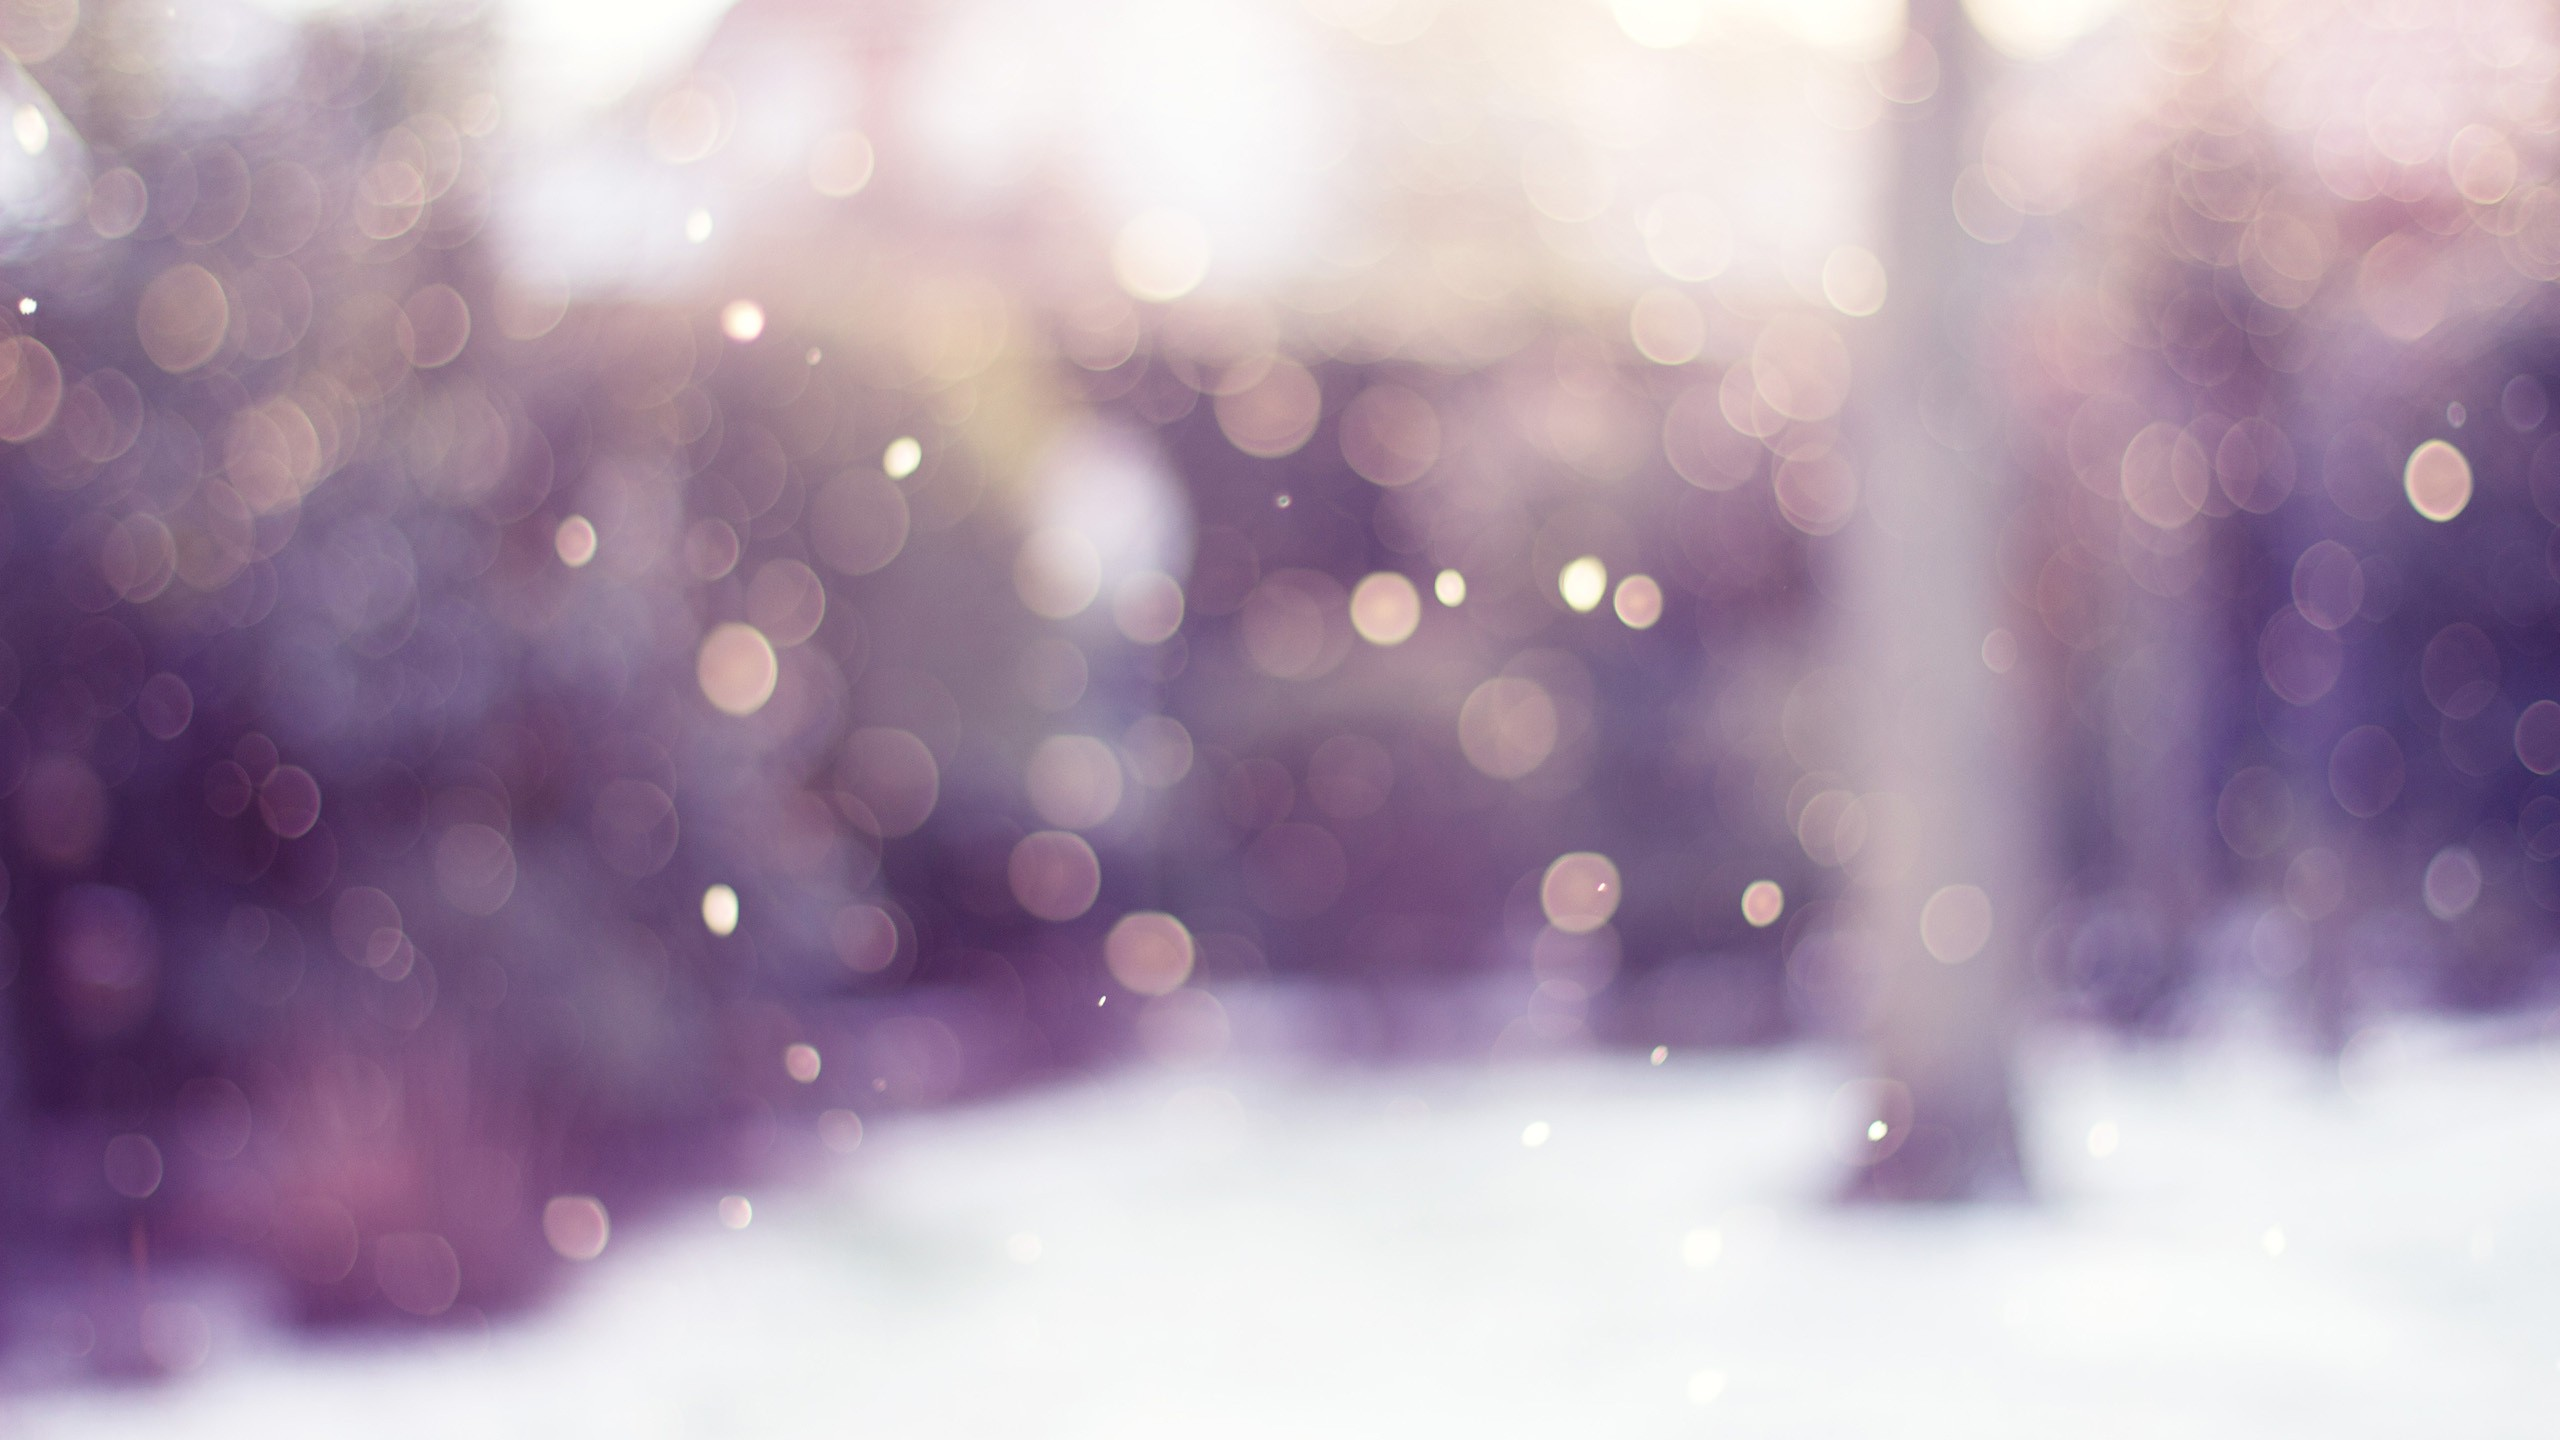
\includegraphics[width=\paperwidth,height=\paperheight]{img/blurry4.jpg}}
\begin{frame}
\begin{center}

\textbf{LATTICE?}
\end{center}
\end{frame}

% VECTOR SPACE
\fontsize{16pt}{15.2}\selectfont
\usebackgroundtemplate{}
\begin{frame}

A bit like a \textbf{vector space}.\vspace{1cm}

\begin{tikzpicture}[scale=.45]
\draw [lightgray] [<->] (0,5) -- (10,5);
\draw [lightgray] [<->] (5,10) -- (5,0);
\draw [thick,purple] [->] (5,5) -- (6, 8);
\draw [thick,purple] [->] (5,5) -- (6, 6);
\pause
\draw [thick,black] [->] (11,5) -- (12,5);

\draw [lightgray] [<->] (13,5) -- (23,5);
\draw [lightgray] [<->] (18,10) -- (18,0);
%\path [fill=purple] (18,5) to (20.5,10) to (23,10) to (18,5);
\path [fill=purple] (15.5,0) to (20.5,10) to (23,10) to (13,0);
\end{tikzpicture}\\
\end{frame}

\begin{frame}

\begin{figure}[!h]
\centering
\begin{tikzpicture}[scale=.5]
\draw [lightgray] [<->] (0,5) -- (10,5);
\draw [lightgray] [<->] (5,10) -- (5,0);

\draw [fill,purple] (9,1) circle [radius=0.1];

\draw [fill,purple] (7,1) circle [radius=0.1];
\draw [fill,purple] (8,2) circle [radius=0.1];
\draw [fill,purple] (9,3) circle [radius=0.1];

\draw [fill,purple] (5,1) circle [radius=0.1];
\draw [fill,purple] (6,2) circle [radius=0.1];
\draw [fill,purple] (7,3) circle [radius=0.1];
\draw [fill,purple] (8,4) circle [radius=0.1];
\draw [fill,purple] (9,5) circle [radius=0.1];

\draw [fill,purple] (3,1) circle [radius=0.1];
\draw [fill,purple] (4,2) circle [radius=0.1];
\draw [fill,purple] (5,3) circle [radius=0.1];
\draw [fill,purple] (6,4) circle [radius=0.1];
\draw [fill,purple] (7,5) circle [radius=0.1];
\draw [fill,purple] (8,6) circle [radius=0.1];
\draw [fill,purple] (9,7) circle [radius=0.1];

\draw [fill,purple] (1,1) circle [radius=0.1];
\draw [fill,purple] (2,2) circle [radius=0.1];
\draw [fill,purple] (3,3) circle [radius=0.1];
\draw [fill,purple] (4,4) circle [radius=0.1];
\draw [fill,purple] (5,5) circle [radius=0.1];
\draw [fill,purple] (6,6) circle [radius=0.1];
\draw [fill,purple] (7,7) circle [radius=0.1];
\draw [fill,purple] (8,8) circle [radius=0.1];
\draw [fill,purple] (9,9) circle [radius=0.1];

\draw [fill,purple] (1,3) circle [radius=0.1];
\draw [fill,purple] (2,4) circle [radius=0.1];
\draw [fill,purple] (3,5) circle [radius=0.1];
\draw [fill,purple] (4,6) circle [radius=0.1];
\draw [fill,purple] (5,7) circle [radius=0.1];
\draw [fill,purple] (6,8) circle [radius=0.1];
\draw [fill,purple] (7,9) circle [radius=0.1];

\draw [fill,purple] (1,5) circle [radius=0.1];
\draw [fill,purple] (2,6) circle [radius=0.1];
\draw [fill,purple] (3,7) circle [radius=0.1];
\draw [fill,purple] (4,8) circle [radius=0.1];
\draw [fill,purple] (5,9) circle [radius=0.1];

\draw [fill,purple] (1,7) circle [radius=0.1];
\draw [fill,purple] (2,8) circle [radius=0.1];
\draw [fill,purple] (3,9) circle [radius=0.1];

\draw [fill,purple] (1,9) circle [radius=0.1];
\end{tikzpicture}
\end{figure}
\end{frame}

\begin{frame}
\textbf{LLL}, a lattice basis reduction algorithm
\vspace{1cm}

\begin{tikzpicture}[scale=.45]
\node [above] at (5,10) {\textbf{random basis}};
\draw [lightgray] [<->] (0,5) -- (10,5);
\draw [lightgray] [<->] (5,10) -- (5,0);

\draw [fill,purple,opacity=.4] (9,1) circle [radius=0.1];

\draw [fill,purple,opacity=.4] (7,1) circle [radius=0.1];
\draw [fill,purple,opacity=.4] (8,2) circle [radius=0.1];
\draw [fill,purple,opacity=.4] (9,3) circle [radius=0.1];

\draw [fill,purple,opacity=.4] (5,1) circle [radius=0.1];
\draw [fill,purple,opacity=.4] (6,2) circle [radius=0.1];
\draw [fill,purple,opacity=.4] (7,3) circle [radius=0.1];
\draw [fill,purple,opacity=.4] (8,4) circle [radius=0.1];
\draw [fill,purple,opacity=.4] (9,5) circle [radius=0.1];

\draw [fill,purple,opacity=.4] (3,1) circle [radius=0.1];
\draw [fill,purple,opacity=.4] (4,2) circle [radius=0.1];
\draw [fill,purple,opacity=.4] (5,3) circle [radius=0.1];
\draw [fill,purple,opacity=.4] (6,4) circle [radius=0.1];
\draw [fill,purple,opacity=.4] (7,5) circle [radius=0.1];
\draw [fill,purple,opacity=.4] (8,6) circle [radius=0.1];
\draw [fill,purple,opacity=.4] (9,7) circle [radius=0.1];

\draw [fill,purple,opacity=.4] (1,1) circle [radius=0.1];
\draw [fill,purple,opacity=.4] (2,2) circle [radius=0.1];
\draw [fill,purple,opacity=.4] (3,3) circle [radius=0.1];
\draw [fill,purple,opacity=.4] (4,4) circle [radius=0.1];
\draw [fill,purple,opacity=.4] (5,5) circle [radius=0.1];
\draw [fill,purple,opacity=.4] (6,6) circle [radius=0.1];
\draw [fill,purple,opacity=.4] (7,7) circle [radius=0.1];
\draw [fill,purple,opacity=.4] (8,8) circle [radius=0.1];
\draw [fill,purple,opacity=.4] (9,9) circle [radius=0.1];

\draw [fill,purple,opacity=.4] (1,3) circle [radius=0.1];
\draw [fill,purple,opacity=.4] (2,4) circle [radius=0.1];
\draw [fill,purple,opacity=.4] (3,5) circle [radius=0.1];
\draw [fill,purple,opacity=.4] (4,6) circle [radius=0.1];
\draw [fill,purple,opacity=.4] (5,7) circle [radius=0.1];
\draw [fill,purple,opacity=.4] (6,8) circle [radius=0.1];
\draw [fill,purple,opacity=.4] (7,9) circle [radius=0.1];

\draw [fill,purple,opacity=.4] (1,5) circle [radius=0.1];
\draw [fill,purple,opacity=.4] (2,6) circle [radius=0.1];
\draw [fill,purple,opacity=.4] (3,7) circle [radius=0.1];
\draw [fill,purple,opacity=.4] (4,8) circle [radius=0.1];
\draw [fill,purple,opacity=.4] (5,9) circle [radius=0.1];

\draw [fill,purple,opacity=.4] (1,7) circle [radius=0.1];
\draw [fill,purple,opacity=.4] (2,8) circle [radius=0.1];
\draw [fill,purple,opacity=.4] (3,9) circle [radius=0.1];

\draw [fill,purple,opacity=.4] (1,9) circle [radius=0.1];
\draw [thick,purple] [->] (5,5) -- (7, 9);
\draw [thick,purple] [->] (5,5) -- (6, 8);
\pause
%
\node [above] at (18,10) {\textbf{reduced basis}};
\draw [thick,black] [->] (11,5) -- (12,5);
\node [above] at (11.5,5) {$_{LLL}$};
%

\draw [lightgray] [<->] (13,5) -- (23,5);
\draw [lightgray] [<->] (18,10) -- (18,0);

\draw [fill,purple,opacity=.4] (22,1) circle [radius=0.1];

\draw [fill,purple,opacity=.4] (20,1) circle [radius=0.1];
\draw [fill,purple,opacity=.4] (21,2) circle [radius=0.1];
\draw [fill,purple,opacity=.4] (22,3) circle [radius=0.1];

\draw [fill,purple,opacity=.4] (18,1) circle [radius=0.1];
\draw [fill,purple,opacity=.4] (19,2) circle [radius=0.1];
\draw [fill,purple,opacity=.4] (20,3) circle [radius=0.1];
\draw [fill,purple,opacity=.4] (21,4) circle [radius=0.1];
\draw [fill,purple,opacity=.4] (22,5) circle [radius=0.1];

\draw [fill,purple,opacity=.4] (16,1) circle [radius=0.1];
\draw [fill,purple,opacity=.4] (17,2) circle [radius=0.1];
\draw [fill,purple,opacity=.4] (18,3) circle [radius=0.1];
\draw [fill,purple,opacity=.4] (19,4) circle [radius=0.1];
\draw [fill,purple,opacity=.4] (20,5) circle [radius=0.1];
\draw [fill,purple,opacity=.4] (21,6) circle [radius=0.1];
\draw [fill,purple,opacity=.4] (22,7) circle [radius=0.1];

\draw [fill,purple,opacity=.4] (14,1) circle [radius=0.1];
\draw [fill,purple,opacity=.4] (15,2) circle [radius=0.1];
\draw [fill,purple,opacity=.4] (16,3) circle [radius=0.1];
\draw [fill,purple,opacity=.4] (17,4) circle [radius=0.1];
\draw [fill,purple,opacity=.4] (18,5) circle [radius=0.1];
\draw [fill,purple,opacity=.4] (19,6) circle [radius=0.1];
\draw [fill,purple,opacity=.4] (20,7) circle [radius=0.1];
\draw [fill,purple,opacity=.4] (21,8) circle [radius=0.1];
\draw [fill,purple,opacity=.4] (22,9) circle [radius=0.1];

\draw [fill,purple,opacity=.4] (14,3) circle [radius=0.1];
\draw [fill,purple,opacity=.4] (15,4) circle [radius=0.1];
\draw [fill,purple,opacity=.4] (16,5) circle [radius=0.1];
\draw [fill,purple,opacity=.4] (17,6) circle [radius=0.1];
\draw [fill,purple,opacity=.4] (18,7) circle [radius=0.1];
\draw [fill,purple,opacity=.4] (19,8) circle [radius=0.1];
\draw [fill,purple,opacity=.4] (20,9) circle [radius=0.1];

\draw [fill,purple,opacity=.4] (14,5) circle [radius=0.1];
\draw [fill,purple,opacity=.4] (15,6) circle [radius=0.1];
\draw [fill,purple,opacity=.4] (16,7) circle [radius=0.1];
\draw [fill,purple,opacity=.4] (17,8) circle [radius=0.1];
\draw [fill,purple,opacity=.4] (18,9) circle [radius=0.1];

\draw [fill,purple,opacity=.4] (14,7) circle [radius=0.1];
\draw [fill,purple,opacity=.4] (15,8) circle [radius=0.1];
\draw [fill,purple,opacity=.4] (16,9) circle [radius=0.1];

\draw [fill,purple,opacity=.4] (14,9) circle [radius=0.1];

% vectors

\draw [thick,purple] [->] (18,5) -- (19, 4);
\draw [thick,purple] [->] (18,5) -- (19, 6);
\end{tikzpicture}\\

\end{frame}

% basis
\begin{frame}

\begin{center}
\begin{tikzpicture}
\node at (0,0) {$B = \begin{pmatrix}
\vec{b_1}\\
\vdots\\
\vec{b_n}
\end{pmatrix}$};

\draw [->] (1.5,0) -- (3,0) node [above] {\textbf{LLL}} -- (4.5,0);

\node at (6,0) {$B' = \begin{pmatrix}
\vec{b_1'}\\
\vdots\\
\vec{b_n'}
\end{pmatrix}$};

\end{tikzpicture}
\end{center}

 \pause

\[ \|b_1'\| \leq \|b_2'\| \leq \hdots \leq \|b_i'\| \leq 2^{\frac{n(n-1)}{4(n+1-i)}} \cdot det(L)^{\frac{1}{n+1-i}} \]
\end{frame}

% COPPERSMITH
\fontsize{35pt}{15.2}\selectfont
\usebackgroundtemplate{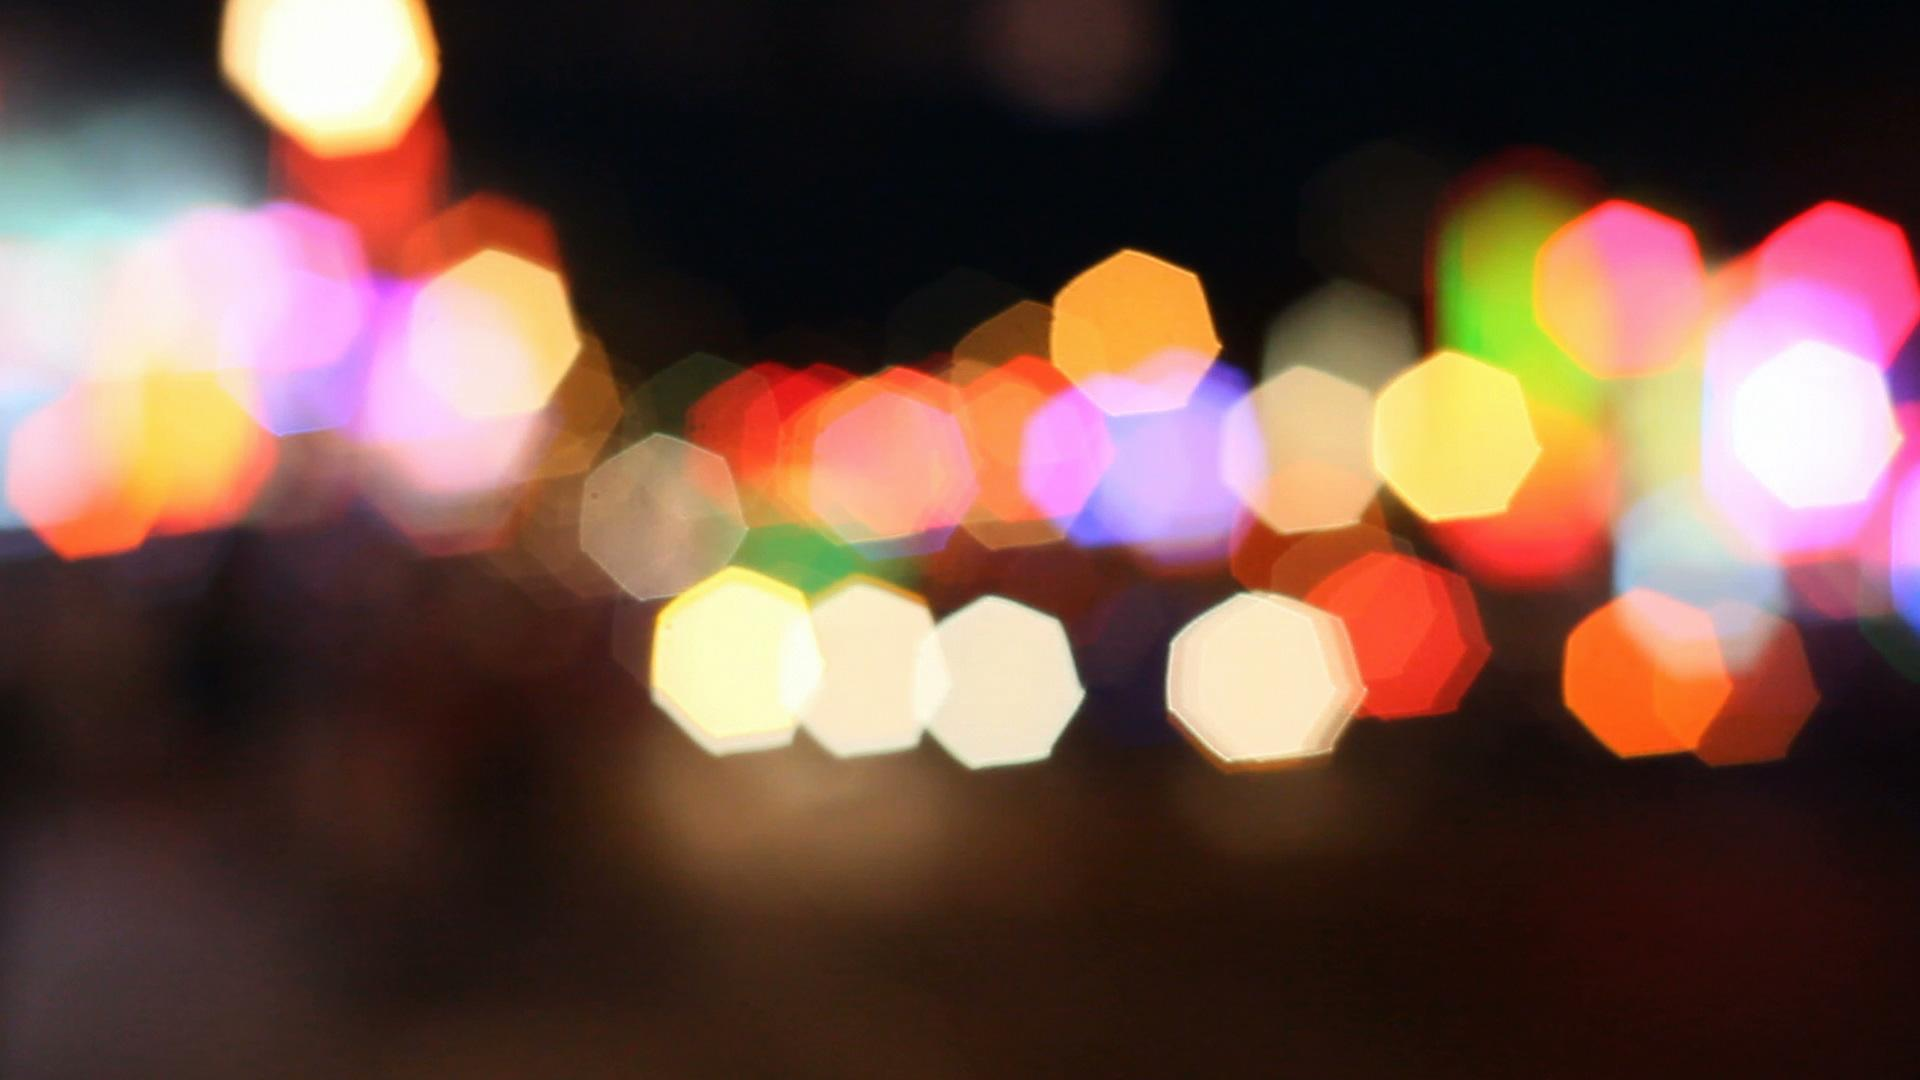
\includegraphics[width=\paperwidth,height=\paperheight]{img/blurry5.jpg}}
\begin{frame}
\begin{center}

\textbf{COPPERSMITH?}
\end{center}
\end{frame}

% VECTOR SPACE
\fontsize{16pt}{15.2}\selectfont
\usebackgroundtemplate{}


% BONEH-DURFEE
\fontsize{90pt}{15.2}\selectfont
\usebackgroundtemplate{
\includegraphics[width=\paperwidth,height=\paperheight]{img/blurry6.jpg}}
\begin{frame}
\begin{center}

\textbf{BONEH-DURFEE?}
\end{center}
\end{frame}

% VECTOR SPACE
\fontsize{16pt}{15.2}\selectfont
\usebackgroundtemplate{}
%
\end{document}